\documentclass[../../main.tex]{subfiles}

%-----------------------------------------------------------%
\begin{document}
\section{Interfacing}
\thispagestyle{fancy}

% Why Interfacing?

% Why are we using FPGA?

% What protocols involved?

% What was used for learning?

% Which sensor was chosen?

% What all do we know about this sensor?

% Why parallel instead of LVDS?

% Block diagram of the flow

% Why 2 SRAMs?

% Possibility of DRAM for storing Star Catalogue

Electrical Interfacing is the interconnection or linking together various aspects of a system together electrically. The major tasks that need to be dealt with are:

\begin{itemize}
    \item {Connection of CMOS sensor with the Controller}
    \item {Proper power to every component}
    \item {Proper interfacing of ports to connect our module with the outside world i.e Satellite}
    \item {Proper Scheduling of every task}
    \item {Software and Hardware design that is able to function as required by Instrumentation, Feature Extraction, Star Matching and Estimation}
    \item {Proper Storage of Image and Star Catalogue for faster processing}
\end{itemize}

% Yash: 
% Dhruv: 
% Siddhi: 

\subsection{Interfacing a Image Sensor with the FPGA}
We began by choosing a cheap camera named OV7670 as a learning task.We have written an AVR code for interfacing it with a micro-controller and also written a VHDL code for interfacing with the FPGA.

For the final task we have chosen the CMOS image sensor named ITS-PYTHON 1300 as the camera.

On studying the datasheet of the python 1300 we came across a protocol named LVDS (low voltage differential signalling) for sending the captured image from the camera to the FPGA. LVDS is communication protocol for high speed communications and is pretty difficult to implement because of the problem of synchronization of the signals sent across the line. Owing to the fact that we do not require such a high speed in our task we decided to go forward with the standard parallel communication protocol.

One portion of our Star Tracker Algorithm consists of image processing on the captured image.  The micro-controller cannot handle the output rate of the image from the Image sensor, thus FPGA, which acts as a buffer, along with external SRAM is being used. % Thus, after pre-processing rest of the task will be done on the micro-controller.

For further coding of this task we have also started learning Verilog in addition to VHDL (Hardware Description Languages) to understand codes online which are in Verilog.

\subsection{Interfacing an SRAM with the FPGA}
SRAM is a type of volatile memory which is static i.e. need not be refreshed from time to time, our system requires a memory module to store and process images coming in from the image sensor, in order to do this we require 2 SRAM modules.

The process is as follows:
\begin{itemize}
    \item The FPGA saves the image bits into the SRAM1.
    \item After the image is stored in SRAM1, it is processed by the FPGA.
    \item In the meantime the second image captured by the image sensor is stored in SRAM2.
    \item So one SRAM acts as an image buffer by storing the incoming image while the other processes the current image at any given time.
\end{itemize}

The SRAM module to be used is not decided yet so we work with the \textit{IS64WV5128BLL/BLS} 512K \(\times\) 8 High-Speed Asynchronous CMOS Static RAM module as reference, the datasheet of which was read and studied.

Accessing data from external memory devices requires data, address and control signals to be asserted in a specific order and held for a specific time following certain timing constraints. These constraints are described in timing diagrams.

We use an asynchronous SRAM since its working is far simpler than its synchronous counterpart, in order to interface our asynchronous SRAM with the FPGA we need to design a memory controller which is responsible for generating the properly timed signals and making the SRAM look ’synchronous’.\\


\subsection{Learning}
\begin{itemize}
    \item Interfacing code of ADC-DAC in VHDL: Interfacing of SRAM involves timing diagrams having timing constraints. Since interfacing of ADC also involves timing constraints, we chose to write code for ADC-DAC interface to gain expertise in this area.
    
    We learnt how to implement sequential logic in VHDL at RTL(Register-Transfer Level). We used FSM (Finite State Machine-way of designing hardware circuits) to build our interface code. We got to learn about usage of counters to fulfill the timing constraints. Our knowledge in VHDL is also enhanced.
    \item High Level Synthesis (HLS) workflow: We perform HLS to convert C-code in to VHDL code. We used `Xilinx Vivado HLS', which is a software to perform HLS. Conversion of code is done by software. The following steps need to be followed to convert a C/C++ project to get it running on an FPGA:
    \begin{itemize}
        \item Modify C-code to run properly in RTL. We add interface pragmas, decide data types which are compatible with HLS (e.g hls::stream for input array etc.).
        \item Once C-code is ready we perform C-synthesis. This step is conversion of the C code to VHDL/Verilog as required.
        \item Next comes C/RTL co-simulation. This is where the generated VHDL/Verilog code is run and the output is matched via the Testbench. 
        \item If everything is working as expected, we export the RTL as an IP Core, which will later be used for designing in Vivado HLx.
        \item We are done with HLS, now we create a new project in Vivado and create a block design for our project.
        \item Import the IP core exported from the appropriate repository and add it to the block design using IP intergrator.
        \item After creating block design, we add the IP cores according to our block-diagram and run connection automation. We can also customise existing IP Cores by  clicking on the block of IP.(e.g. We can have single/dual port BRAM).
        \item On completing our block design, we validate the design. We create an HDL wrapper for our design and then generate the bitstream to program our FPGA.
        \item Finally, we export our hardware and launch SDK. SDK is a tool for testing the output of FPGA using embedded C, which is basically what is used to program the micro-controller.
        \item At this stage, it is recommended to compare timings of the block using software as well as hardware. The software part can be done by simply copy-pasting the function used for HLS and getting its output and verifying it with the hardware output. If pragmas are used correctly, you can expect to see a significant boost in the time to run it on hardware.
    \end{itemize}
    
    \begin{Flowchart}
    \centering
    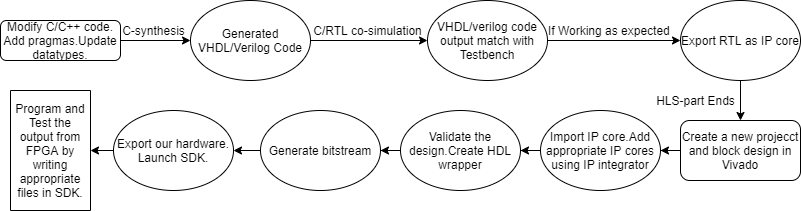
\includegraphics[width=\textwidth]{Figures/Electrical/HLS_Workflow.png}
    \caption{HLS-Workflow}
    \label{FC:hls_workflow}
\end{Flowchart}

  
\end{itemize}
%----------------------------END----------------------------%
\end{document}